%\documentclass[11pt,a4paper]{report}
\documentclass{article}
\usepackage[top=1in, bottom=1in, left=1in, right=1in]{geometry}

%%%%%%%%%%%%%%%%
%%% PACKAGES %%%
%%%%%%%%%%%%%%%%

\usepackage{amsmath}
\usepackage{graphicx}
\usepackage{parskip}

% used with figures:
\usepackage{float}
\usepackage{caption}
\usepackage{subcaption}

\graphicspath{{./img/}}


%%%%%%%%%%%%%
%%% INFOS %%%
%%%%%%%%%%%%%

\title{computer gestuurde regeltechnieken - Part I}
\author{Willem Melis (r0348639)}
\date{\today}

\setcounter{MaxMatrixCols}{20}

%%%%%%%%%%%%%%%%
%%% DOCUMENT %%%
%%%%%%%%%%%%%%%%

\begin{document}

\begin{titlepage}
\begin{center}


\includegraphics[width=3cm]{kuleuven.jpg}~\\[1cm]
\vfill


\textsc{\LARGE KU Leuven}\\[0.7cm]

\textsc{\Large Computer gestuurde regeltechnieken}\\[0.7cm]
\textsc{\Large Exercises - Part 1 }\\[0.7cm]



\centering \huge \bfseries Case study: Quadcopter

\end{center}

\vfill

% auteurs et tuteur
\begin{center}
\emph{Author:} \\[.2cm]
\begin{tabular}[h]{rl}
Willem \textsc{Melis} & r0348639\\
\phantom{------------------------} & \phantom{------------------------}\\
\end{tabular}
\end{center}

\vfill

\begin{center}
\begin{tabular}[h]{rl}
\emph{Professor:} & Bart \textsc{De Moor} \\
\emph{Assistants:}&  
Oscar Mauricio  \textsc{Agudelo} \\
&  Supinya  \textsc{Piampongsant} \\
\phantom{------------------------} & \phantom{------------------------}\\
\end{tabular}
\end{center}

\vfill
\vfill
\vfill

%date
\begin{center} 
2016 - 2017 \\[.5cm]
{\Large \today}
\end{center}

\end{titlepage}

\tableofcontents 
\newpage

\section{Introduction}
The report tries to follow the order of the assignment as much as possible. For each part there is Matlab code, the appendix briefly explains which files belong to which part of the report. Some of the figures are added as an appendix. The text specifically refers to them when the reader should take a look at them, they are of little value on there own.
\section{Linearizion}

\subsection{Find equilibrium point}

Find the fix point with $$x=y=z=\phi=\theta=\psi=0$$

If the system is filled out with these parameters a much simpler set of equations is obtained:

\begin{eqnarray}
\dot{x}=v_x \\
\dot{y}=v_y \\
\dot{z}=v_z \\
\dot{v_x}=-\frac{k \ d}{m}v_x \\
\dot{v_y}=-\frac{k \ d}{m}v_y \\
\dot{v_z}=-\frac{k \ d}{m}v_z -g + \frac{K \ C_m}{m}(v_1^2+v_2^2+v_4^2+v_4^2)\\
\dot{\phi}=w_x \\
\dot{\theta}=w_y \\
\dot{\psi}=w_z \\
\dot{w_x}=\frac{L \cdot k \cdot C_m}{I_{xx}}(v_1^2 - v_3^2) - \frac{I_{yy}-I_{zz}}{I_{xx}} w_y  w_z \\
\dot{w_y}=\frac{L \cdot k \cdot C_m}{I_{xx}}(v_2^2 - v_4^2) - \frac{I_{zz}-I_{xx}}{I_{yy}} w_y  w_z\\
\dot{w_z}=\frac{b \cdot C_m}{I_{yy}}(v_1^2-v_2^2+v_3^2-v_4^2) - \frac{I_{xx}-I_{yy}}{I_{zz}}w_y  w_z
\end{eqnarray}

Its very clear from the that $v_x,v_y,x_z,w_x,w_y$ and $w_z$ are zero ,the remaining equations are set equal to zero :

\begin{eqnarray}
\dot{v_z}= -g + \frac{K \ C_m}{m}(v_1^2+v_2^2+v_4^2+v_4^2) =0\\
\dot{w_x}=\frac{L \cdot k \cdot C_m}{I_{xx}}(v_1^2 - v_3^2) =0 \\
\dot{w_y}=\frac{L \cdot k \cdot C_m}{I_{xx}}(v_2^2 - v_4^2) =0\\
\dot{w_z}=\frac{b \cdot C_m}{I_{yy}}(v_1^2-v_2^2+v_3^2-v_4^2) =0
\end{eqnarray}

simplify even further:

\begin{eqnarray}
g =  \frac{K \ C_m}{m}(v_1^2+v_2^2+v_4^2+v_4^2)\\
v_1^2 - v_3^2 =0 \\
v_2^2 - v_4^2 =0\\
v_1^2-v_2^2+v_3^2-v_4^2 =0
\end{eqnarray}

This means that
\begin{eqnarray}
v_1^2 = v_3^2 \\
v_2^2 = v_4^2 \\
\end{eqnarray}

combine this with the last equation:

\begin{equation}
v_1^2=v_2^2=v_3^2=v_4^2
\end{equation}

This is to be expected as the motors should all be running at the same speed to Hoover. The speed at which these motors need to rotate depends on the gravity which is the last equation $$g =  \frac{K \ C_m}{m}(v_1^2+v_2^2+v_4^2+v_4^2) \\$$ As all the voltages are exactly the same this becomes: $$\frac{m \cdot g}{K \cdot C_m \cdot 4}=   v_i^2 = u_i \\$$ with $i=1...4$

and: $$v_1^2+v_2^2+v_3^2+v_4^2=\frac{m \cdot g}{K \cdot C_m}$$ 

\subsection{Define linear model}

The lineare model is of the form $$\triangle \dot{x}=A\triangle x + B\triangle u $$ $$ \triangle y=C\triangle x$$

The matrix is the Jacobian related to x and matrix B is the Jacobian related to u both evaluated in the equilibrium point.

$$x=[x \ y \ z \ v_x \ v_y \ v_z \ \phi \ \theta \ \psi w_x w_y w_z]  $$
$$x_{equilibrium} = [0\ 0\ 0\ 0\ 0\ 0\ 0\ 0\ 0\ 0\ 0\ 0]$$

$$
u_{equilibrium} =
 [\frac{m \cdot g}{K \cdot C_m \cdot 4} \frac{m \cdot g}{K \cdot C_m \cdot 4} \frac{m \cdot g}{K \cdot C_m \cdot 4} \frac{m \cdot g}{K \cdot C_m \cdot 4}] 
$$

$$
A(x_{equilibrium}) =
\begin{bmatrix}
0 & 0 & 0 & 1 & 0 & 0 & 0 & 0 & 0 & 0 & 0 & 0 \\
0 & 0 & 0 & 0 & 1 & 0 & 0 & 0 & 0 & 0 & 0 & 0 \\
0 & 0 & 0 & 0 & 0 & 1 & 0 & 0 & 0 & 0 & 0 & 0 \\

0 & 0 & 0 & -\frac{k_d}{m} & 0 & 0 & 0 & g & 0 & 0 & 0 & 0 \\
0 & 0 & 0 & 0 & -\frac{k_d}{m} & 0 & -g & 0 & 0 & 0 & 0 & 0 \\
0 & 0 & 0 & 0 & 0 & -\frac{k_d}{m} & 0 & 0 & 0 & 0 & 0 & 0 \\

0 & 0 & 0 & 0 & 0 & 0 & 0 & 0 & 0 & 1 & 0 & 0 \\
0 & 0 & 0 & 0 & 0 & 0 & 0 & 0 & 0 & 0 & 1 & 0 \\
0 & 0 & 0 & 0 & 0 & 0 & 0 & 0 & 0 & 0 & 0 & 1 \\

0 & 0 & 0 & 0 & 0 & 0 & 0 & 0 & 0 & 0 & 0 & 0 \\
0 & 0 & 0 & 0 & 0 & 0 & 0 & 0 & 0 & 0 & 0 & 0 \\
0 & 0 & 0 & 0 & 0 & 0 & 0 & 0 & 0 & 0 & 0 & 0
\end{bmatrix}
$$



$$
u = [u_1 \ u_2 \ u_3 \ u_4] = [v_1^2 \ v_2^2 \ v_3^2 \ v_4^2 ]
$$

$$
B(u_{equilibrium}) = 
\begin{bmatrix}
0 & 0 & 0 & 0 \\ %x
0 & 0 & 0 & 0 \\ %y
0 & 0 & 0 & 0 \\ %z

0 & 0 & 0 & 0 \\ %vx dot
0 & 0 & 0 & 0 \\ %vy dot
\frac{k c_m}{m} & \frac{k c_m}{m} & \frac{k c_m}{m} & \frac{k c_m}{m} \\

0 & 0 & 0 & 0 \\
0 & 0 & 0 & 0 \\
0 & 0 & 0 & 0 \\

\frac{L K c_m }{I_{xx}} & 0 & -\frac{L K c_m }{I_{xx}} & 0 \\
0 & \frac{L K c_m }{I_{yy}} & 0 & -\frac{L K c_m }{I_{yy}} \\
\frac{b c_m }{I_{zz}} & -\frac{b c_m }{I_{zz}} & \frac{b c_m }{I_{zz}} & -\frac{b c_m }{I_{zz}}\\
\end{bmatrix}
$$


\section{discretization}
\subsection{options}
The 3 options are zero-order hold, Euler's rule and the bilinear transformation. (using a sampling time of $T_s=0.05s$). The matrix A is not invertible which means that the zero and hold is not viable. 

\subsection{choice discretization rule}
The bilinear transformation always maps stable poles in the continuous domain to stable poles in the discrete domain. However in this particular case both Euler and the bilinear transformation have stable poles. The are both fully controllable and observable. The only real difference is in the transmission zeros, the  bilinear transformation has transmission zeros while Euler does not. This makes the  bilinear transformation the preferred choice in this case. As transmission zeros are stable which means the system is minimum phase system as the 8 transmission zeros are all -1 which is inside the unit circle.
\section{LQR controller with payload}
\subsection{full-state feedback controller}

The controller is constructed in Simulink (Figure~\ref{fig:simulink diagram full-state feedback controller}) according to the diagram on page 221 of the course notes. 

\begin{figure}[H]
	\centering
	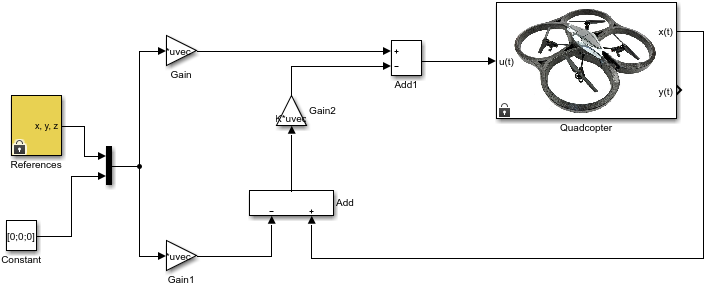
\includegraphics[width=0.5\textwidth]{./LQG/full_state_feedback_simu.png}
	\caption{simulink diagram full-state feedback controller}
	\label{fig:simulink diagram full-state feedback controller}
\end{figure}

The matrix K is calculate with the LQR method as we did in the second exercise session. However in order to do LQR we need a matrix Q and R. As LQR minimizes $J_N = \frac{1}{2} \sum_{k=0}^{N-1}[x_k^TQx_k + u^T_kRu_k] + \frac{1}{2}x_N^TQx_N$. Notice how Q determines the weights given to $x_k$ and and R determines the weights given to $u_k$. 

If Q and R are taken as an diagonal matrix with ones on the diagonal then the quad copter does not have enough power to stay in the air. This is displayed in Figure~\ref{fig:full-state controller with simple diagonal matrices as Q and R}. Its very clear from Figure~\ref{fig:full-state controller with simple diagonal matrices as Q and R demo bad z position} that the controller does not optimize enough on the z axis.

\begin{figure}[H]
	\centering
	\begin{subfigure}[b]{0.3\textwidth}
		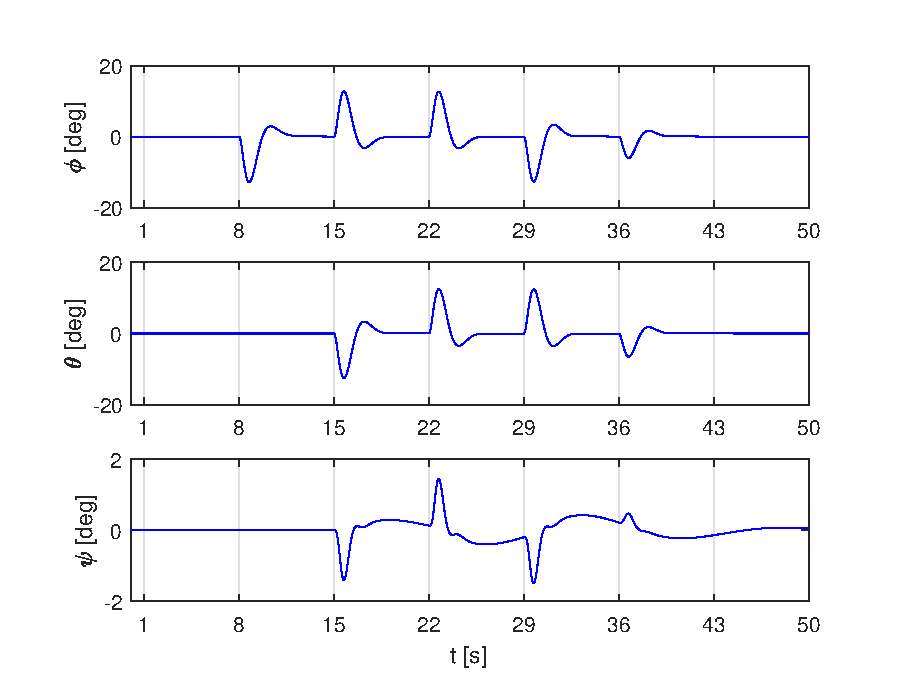
\includegraphics[width=\textwidth]{./LQG/full_state_feedback_first_fig4.eps}
		\caption{angels}
	\end{subfigure}
	\begin{subfigure}[b]{0.3\textwidth}
		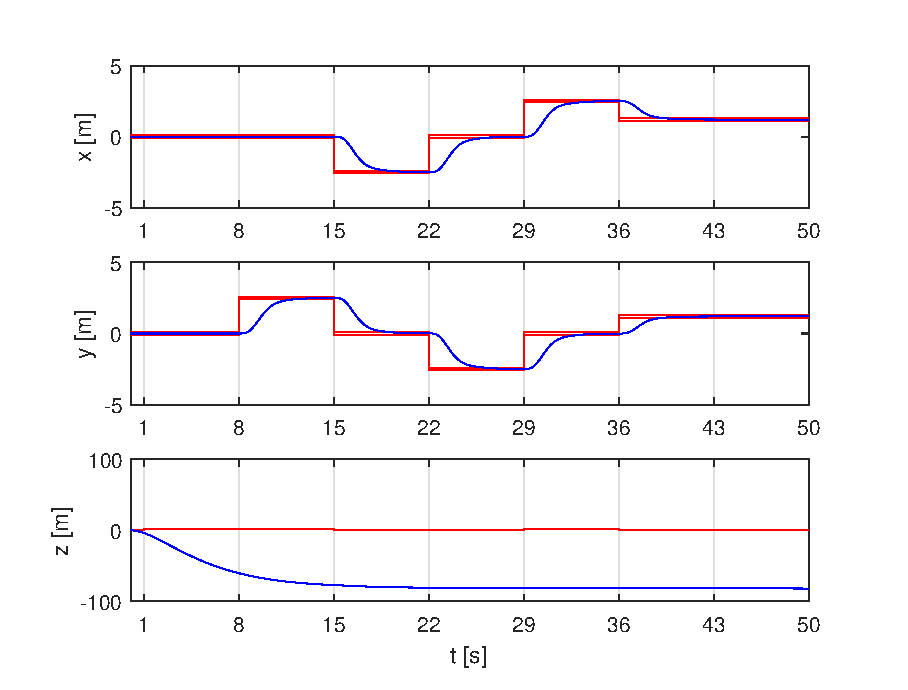
\includegraphics[width=\textwidth]{./LQG/full_state_feedback_first_fig3.eps}
		\caption{position}
		\label{fig:full-state controller with simple diagonal matrices as Q and R demo bad z position}
	\end{subfigure}
	\begin{subfigure}[b]{0.3\textwidth}
		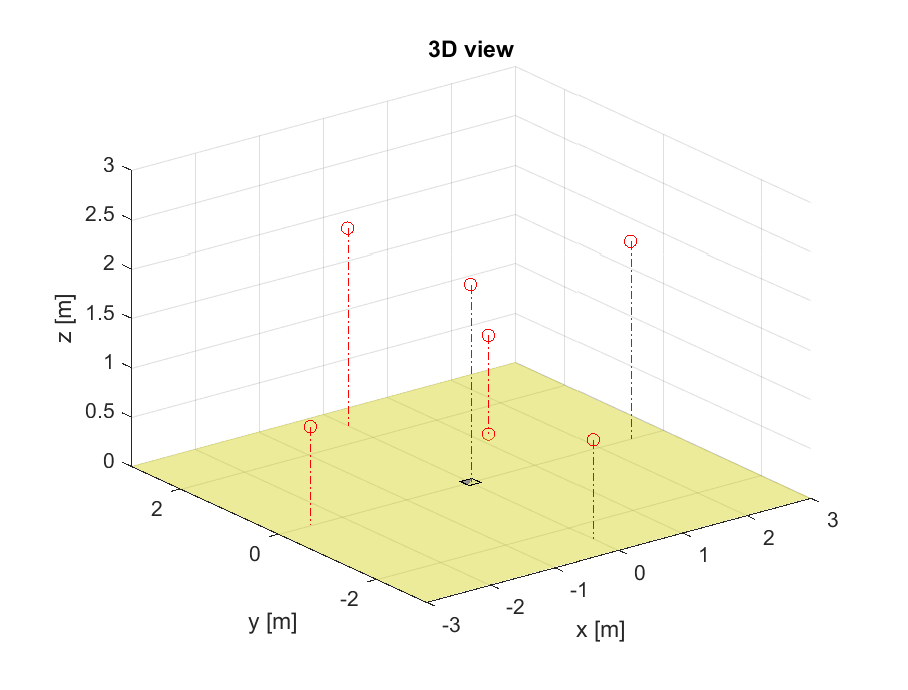
\includegraphics[width=\textwidth]{./LQG/full_state_feedback_first_fig2.eps}
		\caption{position}
	\end{subfigure}
	\caption{full-state controller with simple diagonal matrices as Q and R}\label{fig:full-state controller with simple diagonal matrices as Q and R}
\end{figure}

In order to get a proper controller we need to put way more weight on the position z in the optimization problem. This is done by increasing a value in Q, as the z coordinate is an state. 

$$ 
Q=
\begin{bmatrix}
1 & 0 & 0 & ... \\
0 & 1 & 0 & ...\\
0 & 0 & 1 & ... \\
... & ... & ... & ... 
\end{bmatrix}
=>
\begin{bmatrix}
1 & 0 & 0 & ...\\
0 & 1 & 0 & ...\\
0 & 0 & 10^{7} & ... \\
... & ... & ... & ... 
\end{bmatrix}
$$

\begin{figure}[H]
	\centering
	\begin{subfigure}[b]{0.3\textwidth}
		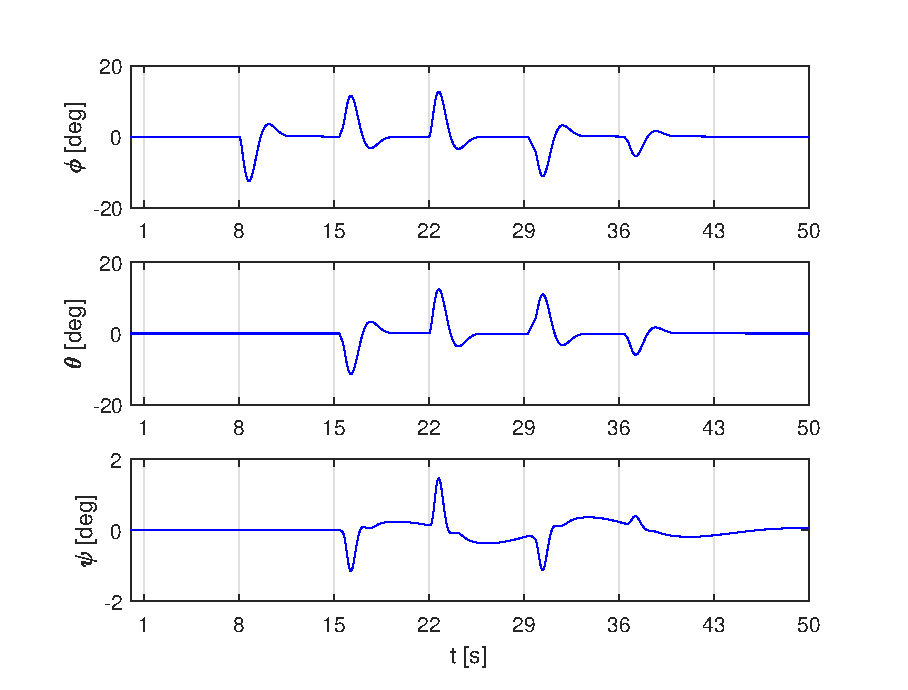
\includegraphics[width=\textwidth]{./LQG/full_state_feedback_final_fig4.eps}
		\caption{angels}
	\end{subfigure}
	\begin{subfigure}[b]{0.3\textwidth}
		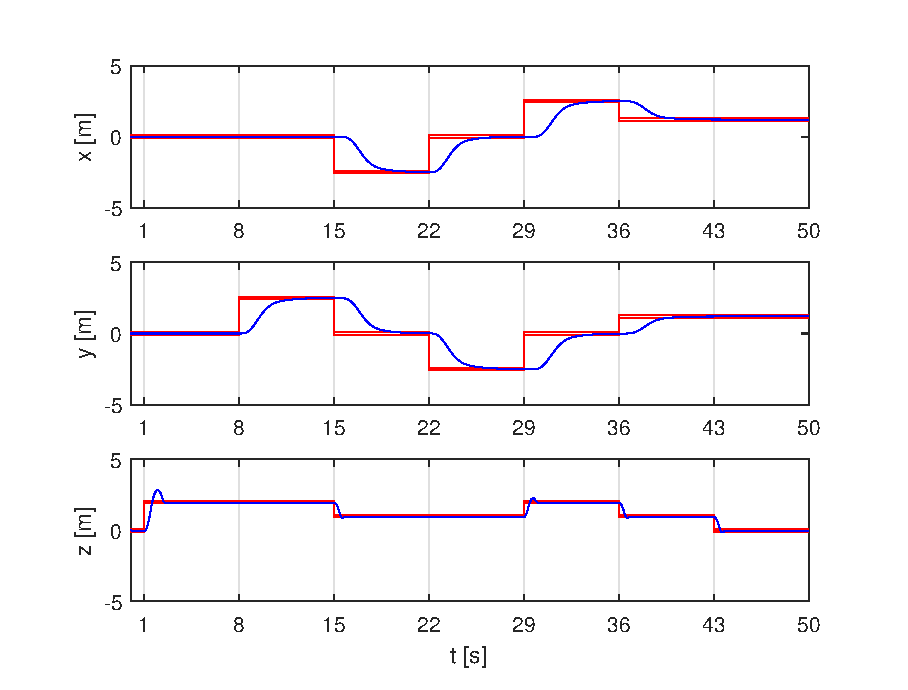
\includegraphics[width=\textwidth]{./LQG/full_state_feedback_final_fig3.eps}
		\caption{position}
	\end{subfigure}
	\begin{subfigure}[b]{0.3\textwidth}
		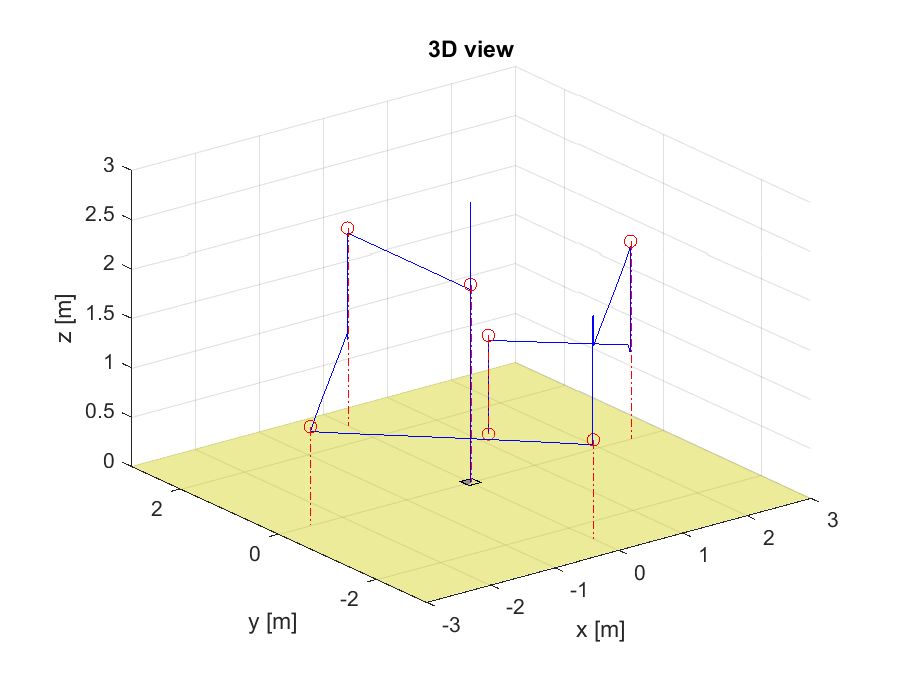
\includegraphics[width=\textwidth]{./LQG/full_state_feedback_final_fig2.eps}
		\caption{position}
	\end{subfigure}
	\caption{full-state controller with proper diagonal matrices as Q and R}\label{fig:full-state controller with proper diagonal matrices as Q and R}
\end{figure}
\subsection{LQR controller with integral action}

\subsection{discussion both results}
\section{LQR controller without payload}


% \appendix
% \section*{Codes}
% \addcontentsline{toc}{section}{Codes}
% \input{appendix/code.tex}

\end{document}
